\documentclass{ledger}

%AUTHOR: This is a bare-bones template into which you may put your paper to aid in formatting your submission to Ledger. Note that to work properly, you must have the files "ledger.cls", "ledgerbib.bst", and the folder "images" on hand. 

%AUTHOR: the preferred method to generate PDF output is to use 'pdflatex'
%To clean up after a successful build, try: 'latexmk -c main.tex'


%EDITOR: replace X's to set the data for the header and footer
\newcommand{\thefirstpagenum}[0]{X}
\newcommand{\thelastpagenum}[0]{X}
\newcommand{\theyear}[0]{20XX}
\newcommand{\thevol}[0]{X}
\newcommand{\thedoi}[0]{DOI 10.5195/LEDGER.\theyear.XXX}
\newcommand{\ledgerpages}[0]{\thefirstpagenum-\thelastpagenum}


%AUTHOR: please set these to generate correct PDF metadata
\hypersetup{pdfauthor={Pisano, Matthew T.; 
Patterson, Connor J.}, pdftitle={PredictChain}}

%EDITOR: set the correct pageination during layout
%\setcounter{page}{\thefirstpagenum}


%AUTHOR: this can be used to highlight changed text, surround with \edit{} and
%uncomment either to determine color
%\newcommand{\edit}[1]{{\color{red} #1}}
\newcommand{\edit}[1]{#1}
	
\overfullrule=10pt

\title{PredictChain:\\
A Blockchain-based Predictive Marketplace}
\author{
    Matthew T. Pisano,\thanks{BTC/BCH/ETH ADDRESS}\thanks{M. T. Pisano (pisanm2@rpi.edu.edu) is a graduate
    student at Rensselaer Polytechnic Institute.} 
    Connor J. Patterson,\thanks{C. J. Patterson (pattec3@rpi.edu) is an undergraduate student at
    Rensselaer Polytechnic Institute.}
}

\pagestyle{pagemain}


%The Author should select the appropriate pretitle below:
\pretitle{
  %\centering \selectfont LEDGER \LaTeX \ TEMPLATE \par
  %\centering \selectfont REVIEW ARTICLE \par
  \centering \selectfont RESEARCH ARTICLE \par 
  \fontsize{24pt}{28pt}\selectfont} % Title is centered and at 24pt


\begin{document}

\maketitle

\thispagestyle{pagefirst}

\begin{abstract}
The accessibility of resources for artificial intelligence (AI) model training and development is a significant issue
in research. Limited access to computing resources and predictive training data impedes individuals and groups from
training predictive models on their data. The entities with the required computational resources often keep the results
of their trained models private, which results in inefficiency and the withholding of useful predictions from the
general public. Despite the existence of many pre-trained and open source models, it is likely that these few, available
models will not fit someone's particular needs. To address these issues, we propose a blockchain-based marketplace called
PredictChain for predictive AI models. Users can upload datasets to train predictive models, request to train models on
previously uploaded datasets or submit queries to trained models. A central node with available computing resources will
operate these models with varying archetype models, from cheap, fast, and simple to more expensive, slower, and more
powerful. This central-node architecture will simplify the process of gathering the compute needed for operating this
project, as only one node is required.  This approach would enable users to create better models that are open to the
public for usage and promote data sharing, thus opening up the AI industry to the masses and reducing dependence on
centralized tech giants. This project, with sufficient participation, can significantly improve the accessibility of
machine learning, which currently poses a challenge to most people.

% This project would serve to open up this black box of industry and encourage the sharing of datasets and parameter configurations to create better models that are open to the public for usage.

%AUTHOR: keywords are OK to show for Review article, will be hidden and added to metadata for publication
\begin{keywords}
\item Bockchain.
\item Decentralized.
\item Marketplace.
\item Oracle.
\item LSTM.
\item GRU.
\item RNN.
\end{keywords}
\end{abstract}


\section{Introduction}

Artificial intelligence (AI) has become an essential part of our lives, from voice assistants to self-driving cars.
However, the development and training of AI models require enormous amounts of data and computing resources. This
limitation has led to the concentration of AI development in the hands of a few large tech companies, which creates an
obstacle to innovation and hinders progress in the field. Furthermore, the lack of transparency and accessibility in the
industry means that many people cannot utilize the benefits of AI in their own work and research.
Decentralized AI marketplaces have emerged as promising solution to these challenges. These marketplaces allow individuals
and organizations to share their data and computational resources to develop and train AI models collectively. By leveraging
blockchain technology, decentralized AI marketplaces can facilitate secure, transparent, and decentralized access to AI
models and data, promoting innovation and collaboration across the field.
In this paper, we explore the need for a decentralized AI marketplace, examining the limitations of the current
centralized approach to AI development and training. We propose a blockchain-based marketplace, which we call
``PredictChain,'' that aims to democratize access to AI models and training data.

PredictChain helps to solve one of the main issues that involve AI models today: accessibility.
Oftentimes, individuals or groups pose data that they would wish to be used in predictive analysis.
However, these people may not have access to the computing capacity needed to train predictive models on this data.
Additionally, other people have neither access to predictive training data nor do they have access to computational resources.
When users upload their datasets to PredictChain, they allow a model to be trained on the datasets uploaded.  To avoid \
restrictions data is not stored on the blockchain directly, rather in other locations, outlined in the
\hyperref[subsec:oracle]{Oracle} subsection below. Higher-quality datasets will produce higher-quality models.
When users submit parameters for training, they allow the model that their parameters produce to be used publicly.
Both of these users are rewarded for their work when a model is queried.  The amount of this reward is based on the
correctness of the prediction.  This encourages users to participate in contributing the resources needed for good
predictions while leaving a public record for other users to view.  This is in contrast to large cloud organizations,
such as \textit{AWS} or \textit{Google Cloud}, that allow users to train models on custom datasets as well, but this
comes at a price, with no chance of reward if a model does well.

As the scale and power of AI models grow, the resources required to train them also grow.  This makes the training of
useful machine learning models unattainable for most people.  To get useful results from these models, users often have
to pay large, centralized organizations without any reward if they provide a good dataset or model parameters.
PredictChain changes this paradigm by incentivizing the thoughtful creation of useful models and datasets.
The PredictChain marketplace allows individuals and organizations to share their data and computational resources, which
can then be used to train AI models collaboratively. The blockchain acts as a secure and transparent ledger that facilitates
transactions between participants in the marketplace, enabling them to exchange resources in a trustless and decentralized manner.
In this model, participants can contribute their unused computing power to the marketplace, and in exchange, they receive
ALGO tokens that represent their contribution. These tokens can then be used to access computing resources from other
participants in the marketplace or to purchase AI models that have been trained on the data contributed by other participants.


\section{Background on the Blockchain Platform Used for PredictChain}

After the recent hype and subsequent crashes around cryptocurrencies that are powered by blockchain technologies, we
should not forget that blockchain can be used for genuine utility in addition to cryptocurrencies and investment
opportunities~\cite{crosby2016blockchain}.  Blockchain technologies provide several advantages for this type of
marketplace. Firstly, it enables participants to exchange resources without needing a centralized intermediary, reducing
transaction costs and promoting decentralization. Secondly, it provides a secure and transparent record of all
transactions, enhancing trust and reducing the risk of fraud or manipulation. Finally, it enables participants to
maintain control over their data and computing resources, ensuring that they are not used without their permission or
in a manner that violates their privacy or security.

In our work, we utilize the Algorand Blockchain~\cite{gilad2017algorand} as a testbed for PredictChain.  The Algorand
blockchain is a decentralized, permissionless, and high-performing blockchain well-suited for creating a decentralized
AI marketplace. First, Algorand's unique Pure Proof of Stake (PPoS) consensus algorithm~\cite{dimitri2022proof} and
architecture provides several advantages that make it an ideal choice for this type of application. The PPoS consensus
algorithm ensures fast and secure transaction processing, enabling rapid and efficient transactions within the marketplace.
This means that participants can quickly and easily exchange resources without needing a centralized intermediary,
reducing transaction costs and promoting decentralization.  Second, Algorand's smart contract capabilities allow for
the creation of custom smart contracts that can be used to govern transactions within the marketplace. Smart contracts
can be used to enforce rules and regulations around the use of data and computing resources, ensuring that participants'
privacy and security are protected.
Third, Algorand's Layer-1 architecture enables the creation of scalable and high-performing applications. The platform
can support many transactions per second, enabling participants to quickly and efficiently exchange resources within the
marketplace.  Finally, Algorand's commitment to sustainability and energy efficiency aligns with the goals of creating
a more environmentally friendly and sustainable AI industry. The platform's low energy consumption and carbon footprint
make it an attractive choice for those seeking to reduce the environmental impact of AI development and training.
Overall, the Algorand blockchain provides a robust and efficient platform for the creation of a decentralized AI
marketplace. Its unique features and architecture make it an ideal choice for this type of application, enabling greater
collaboration and innovation in the field of AI.
Furthermore, by primarily using Algos as a method of payment, it helps to, once again, show that cryptocurrencies can
effectively be used as a pure form of payment for useful services.

\section{Related Work}

\subsection{Sharing Updatable Models}

Decentralized \& Collaborative AI on Blockchain~\cite{sharingModels} is a great example of a project that combines both
artificial intelligence and blockchain technologies in a similar manner to our own.  The authors outline a blockchain-based
predictive marketplace that utilizes AI for predictive analysis. There exists an initial model trained on the data
collaboratively provided by multiple users. To encourage the submission of high-quality data, the authors propose an
incentive mechanism that rewards honest users and punishes dishonest ones.  This model is trained off-chain on the client's
machine.  All the logic involving the data submission and incentives is done within an Ethereum smart contract.

\paragraph{The Model}
This system leaves the exact definition of the model flexible between different clients running the system.  The authors
suggest that the specific class of model would be some type of predictive model, giving examples of CRF-RNNs and Support
Vector Machines.  Depending on the model that is used, the authors mention that the corresponding incentive mechanism
would change from model to model.

\paragraph{Incentives}
Similarly to the models, the authors leave the incentive mechanism of the project also without an exact definition.
This is to give end users flexibility in their individual implementations.  They do give several examples and specifications
of this mechanism, however.  These examples fall into two categories: gamification and monetary incentives.  In the
gamification strategy, they suggest that there should be no monetary incentive for contributing data, instead using
tokens or badges.  For the monetary route, they suggest that users who choose to upload data may have to also submit
some stake into the contract as collateral.

\subsection{The Price You Pay For Trust}

Blockchain Enabled AI Marketplace: The Price You Pay For Trust~\cite{priceOfTrust} is another example of a marketplace
that uses both AI and blockchain technologies effectively.  One of the main focuses of this project is on privacy. It
explicitly gives examples of health or insurance entities needing models trained on confidential data.  The principles
that this project is built around are \textit{trust}, \textit{fairness}, and \textit{auditability}.

\paragraph{Datasets}
The datasets in this system are unique since the bulk of the data is not tied directly to any one training request.
In this project, a user uploads only a small chunk of data.  This data will then be used as the validation set for the
training.  Most of the training data for this query is pulled from private sources.  This serves the purpose of only
requiring users to upload a small portion of their data.  However, this has the disadvantage of requiring external data
to train models.  To accommodate this, the authors implement several layers of security to protect private data sources.

\paragraph{Models}
The models that this paper targets are much less integrated than those of other papers.  Also, unlike other
implementations, these models are trained in a decentralized nature.  This training strategy is reflective of federated
learning.  No one model is given all the data in bulk. It is only given sections with confidential information stripped
out. To add to their security, they also use hashing algorithms to secure their data further.  Additionally, the models
themselves are eventually shared with the requesting user along with the model results.

\paragraph{Blockchain Communication}
Like other projects, this implementation uses a significant off-chain component.  This component communicates with the
private, permissioned blockchain that this system uses.  This allows for more complexities in the training of the models,
as on-chain training has significant speed and memory constraints.  By using Hyperledger Fabric for data distribution,
data can be selectively distributed to only the nodes that need the data for training that will
have access to it.

\subsection{Blockchain Prediction Markets for Renewable Energy}

Towards the Use of Blockchain Prediction Markets on Forecasting Wind Power~\cite{windForcasting} is a paper that lays
the groundwork for a use-case of blockchain-empowered prediction markets. Like blockchain technology, renewable energy
has recently ballooned in use.  This paper combines these two fields in a way that utilizes their combined utility for
aiding progress in the field of renewables.

\paragraph{Motivations}
A key problem with many forms of renewable energy sources is their unpredictable supply. Wind turbines need wind. Solar
panels need sunshine. Being able to better forecast the output of these energy production methods at a various time or
place can help alleviate the pitfalls that prevent them from growing in market share.

\paragraph{Implementation}
On their platform, anyone can propose an event and request predictions for that event with the promise of providing a
reward.  Reporters then propose several predictions over the course of the seven-day window that the market is active.
In this implementation, the hosts of this predictive market do not take responsibility for the training and execution of
the predictive models.  This is all done on the side of the reporters.  Using their framework, reporters who provide
correct data are rewarded, and those who provide inconsistent data are punished.

\subsection{Stock Predictions}

This next paper is closely aligned with the example dataset we use for PredictChain.  They focus on using big data to
train predictive machine learning models to forecast the short-term future behavior of stocks within the Chinese stock
market~\cite{deepPrediction}.  For their dataset, they gathered the past performance of 3558 stocks from the Chinese
stock market over a period of two years.  In order to gather this data, they utilized the \textit{Tushare} API, along
with web-scraping from \textit{Sina Finance} and the \textit{SWS Research} website. Within their paper, they utilize
several techniques; designed to cut down on the noise inherent to the stock market to allow for better predictions.
Their primary method for doing this was through feature engineering.

\paragraph{Feature Engineering}
As part of their feature engineering, they utilized three primary techniques.  First, they applied feature extension to
their dataset.  Through the use of this technique, they added additional meta-attributes to the entries, such as
polarizing or calculating the fluctuation percentage.  Adding this meta-data to the dataset helps to give the model a
more complex picture of the stock and how it performs over time.  Next, they eliminated some features, based on their
influence, by using the Recursive Feature Elimination (RFE) algorithm.  By eliminating unnecessary features, they allow
their model to pay more attention to the most influential features, improving its predictive capabilities.

\paragraph{Predictive Models}
For their testing, the authors used a two-layered LSTM model, with the model only having an input layer and an output
layer.  As for their output, they kept the output as simple as possible to make sure the model was focused only on
predicting the movement of the stock.  The model either outputted a $1$ for the stock going up at a given time step,
or a $0$ if the model believed the stock would go down.


\subsection{Distributed, Decentralized, and Democratized AI}

The authors of this paper have also noticed the problem of accessibility in the realm of artificial intelligence.  Like
our project, their solution was to implement a distributed AI marketplace that utilized blockchain
technologies~\cite{democratizedAI}.  Their marketplace implementation, \textit{SingularityNET}, was designed with the
intention of making AI development and training more accessible to everyone.  In this paper, Montes and Goertzele argue
that this democratization is not only useful for allowing more people to access AI technologies, but it also has a
significant impact when it comes to the development of artificial general intelligence (AGI).

\paragraph{The Dangers of Centralization}  In their work, the authors make a note of the fact that the current development
of artificial intelligence systems is controlled primarily by only a handful of large tech giants, such as Amazon or
Google. They argue that this degree of centralization would have a negative impact on any eventual AGI.  This is due
to the bias that it may be given when trained only by a few thousand individuals, missing out on important data that can
be gathered from outside of these organizations.

\paragraph{A Decentralized Marketplace}  Their solution to this centralization problem is the \textit{SingularityNET}
marketplace.  Here, users can request or provide AI services.  These actions are organized using simple, smart contracts
that take in payment from the requesting users and distribute rewards to service-providing users.  Utilizing blockchain
and smart contract technologies is designed to avoid the closed and centralized qualities that many contemporary AI
marketplaces embody.


\subsection{Evaluation and Analysis}

Through this review, we examined several papers that demonstrate similar ideas and architectures to our project with
slightly different implementations.  Harris and Waggoner (2019)~\cite{sharingModels} had many similarities to our project
but was implemented using a more decentralized architecture.  Sarpatwar et al. (2019)~\cite{priceOfTrust} take some of
the decentralization ideas of Harris and Waggoner (2019)~\cite{sharingModels} and expand upon it by structuring their
project with security as another main focus.  Shamsi and Cuffe (2020)~\cite{windForcasting} demonstrates a market similar
to ours, but using a more decentralized architecture and a more specific scope.  Next, Shen and Shafiq (2020)~\cite{deepPrediction}
helped us to better understand some of the future improvements that we could make to both our dataset preprocessing
and model training.  Finally, Montes and Goertzel (2019)~\cite{democratizedAI} demonstrated a marketplace very similar
to our own, with a greater focus on the larger context around the issue of AI accessibility, its potential consequences,
and its potential solutions.

In our work, we have expanded upon these ideas and addressed some of their shortcomings.  PredictChain features a more
centralized architecture than these papers, Sarpatwar, et al. (2019)~\cite{priceOfTrust} and Shamsi and
Cuffe (2020)~\cite{windForcasting} in particular. Our aim with this strategy is to focus on simplicity and ease of use.
Without the requirement for a large network of oracles, our implementation allows anyone to quickly set up an oracle
instance and begin connecting to clients.  Another design choice that we made was in our suite of built-in archetype
models.  By giving each client a preset list of models to choose from, it is no longer the client's responsibility to
train and implement the models, as in Harris and Waggoner (2019)~\cite{sharingModels}.  This helps to make setup and
usage much cleaner and more accessible.  Overall, PredictChain aims to be more generalized and accessible to non-technical
users at the cost of centralization.

\section{Implementation Details}

The structure of PredictChain is primarily broken up into two parts: the client and the oracle.  Both of these parts
interact with each other through the blockchain.  The following diagram illustrates this relation:

\begin{figure}[H]
    \begin{center}
        \begin{minipage}{0.6\textwidth}
        \centering
        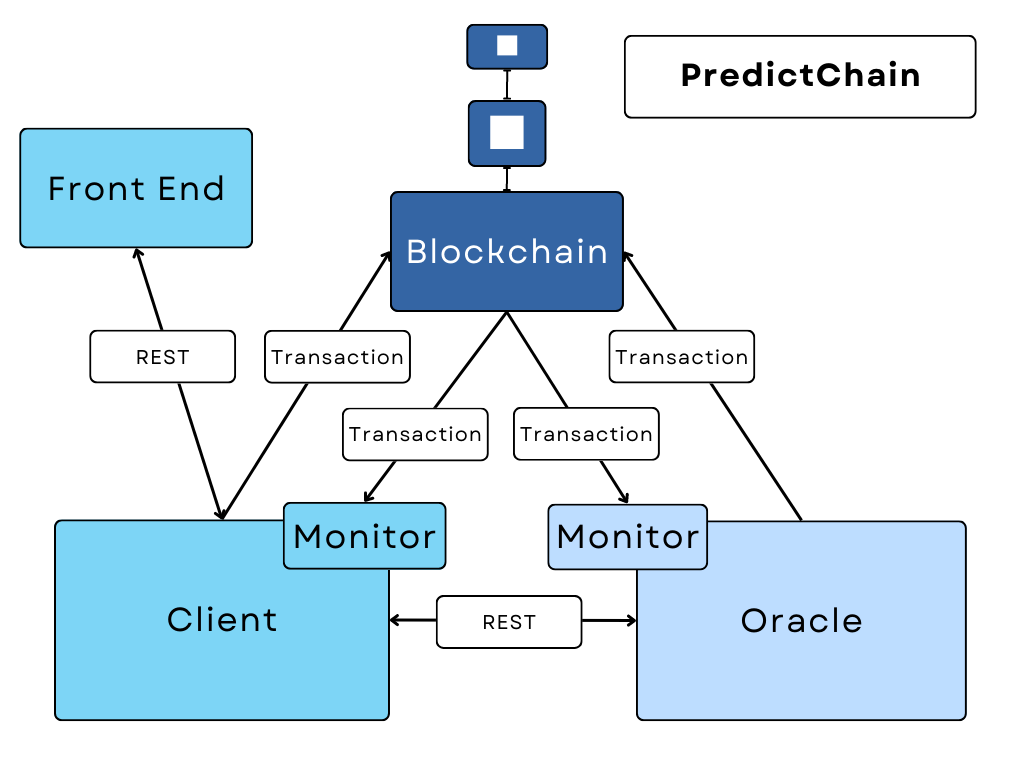
\includegraphics[width=\linewidth]{images/detailedDiagram}
        \caption{The architecture of PredictChain}\label{Fig:detailedDiagram}
    \end{minipage}\hfill
    \end{center}
\end{figure}

The above diagram illustrates the core components of the system, along with their methods of communication.

\subsection{The Front End UI}
Although not directly related to the AI or the blockchain parts of the product, it is still important to discuss the UI
aspect of our project. The UI sets the user's impression of PredictChain by having multiple pages that create a more
pleasant experience for the user. For example, the home page talks about our mission, how we differ from our competitors,
and example model sets we provide. The addition of the \textit{FAQ} and \textit{Meet the Team} pages allows users to
understand who created PredictChain, as well as get answers about any privacy/security concerns they might have. Lastly,
users can create an account or log in to a pre-existing account. Then users are able to use PredictChain to its fullest
functionality such as adding datasets, checking prices, or querying models with provided datasets. The UI talks to the
client through a series of REST requests in order to convey this data, later receiving the result of the user's actions
later through the same means.

\subsection{The Client}

The client serves as a middleman between the front-end user interface and the blockchain.  It is run as a server,
serving UI content to the user, taking in requests from the UI, and parsing those requests into a form suitable for both
the blockchain and for the oracle.  Additionally, the client constantly polls for updates coming from the oracle, through
the blockchain, and then through its monitor.  These updates are queued and sent to the front end upon request. This allows
the user to both interact with the blockchain and to see the important updates that come from it.

\subsection{The Oracle}
\label{subsec:oracle}

The oracle accomplishes the majority of the other tasks that this project requires.  It constantly polls for updates
coming from the client through the blockchain by using its monitor.

\begin{figure}[H]
    \begin{center}
        \begin{minipage}{0.6\textwidth}
        \centering
        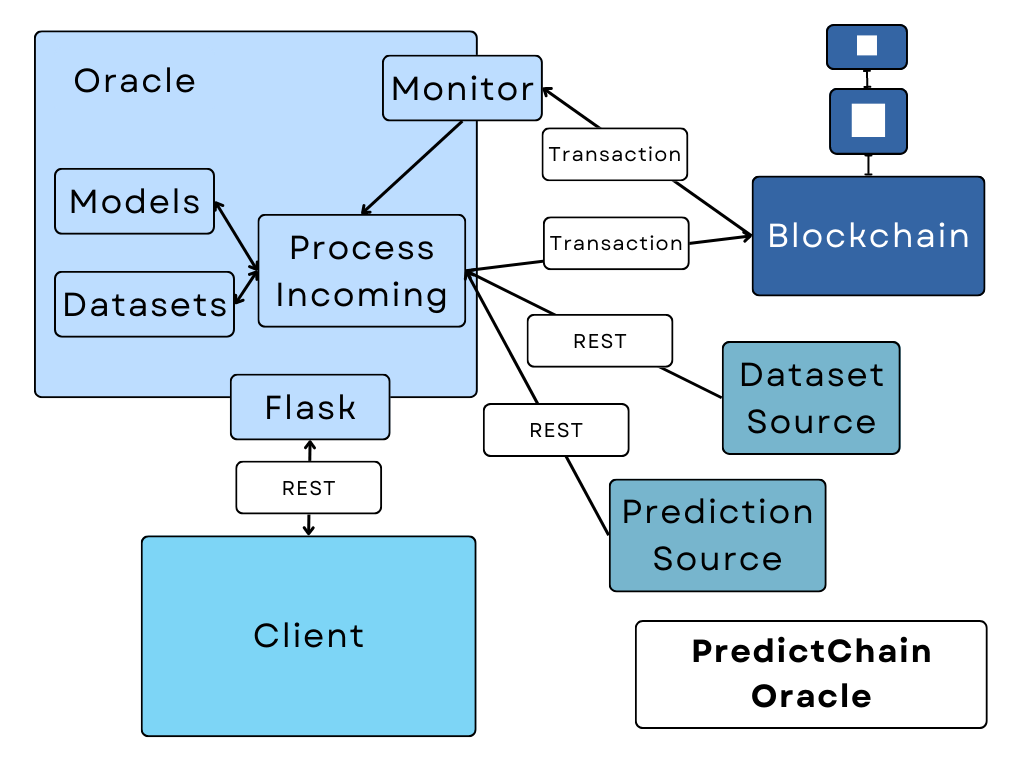
\includegraphics[width=\linewidth]{images/oracleDiagram}
        \caption{The architecture of the Oracle}\label{Fig:oracleDiagram}
    \end{minipage}\hfill
    \end{center}
\end{figure}

Upon receiving these updates, it begins the execution of one of its three main operations.  These are:

\begin{itemize}
    \item Downloading a user-specified dataset and saving it
    \item Training one of the raw models based on user-inputted parameters
    \item Querying one of the trained models on user-inputted data and comparing it to the real-world result
\end{itemize}

After each of these operations, the oracle sends out several blockchain transactions.  These can be either rewards to
contributors of a model or confirmations/results of the operation that has been performed.

When working with user-submitted datasets, the oracle uses a handler to manage the operations performed on that dataset.
The handler can save datasets to a specified environment, load datasets from a specified environment, parse them as a
pandas data frame, and split the dataset by the values of one of its attributes.  The environments that the handler
recognizes are \textit{local} and \textit{IPFS}.  By using saving a dataset locally to the Oracle or uploading it to
\textit{IPFS}, we avoid the restrictions that come with uploading it directly to the Algorand blockchain.  When using
either of these environments, the handler abstracts away the complexities of working with either of them into a unified
interface.

When working with user-trained models, the oracle uses a similar, common interface.  This interface can create the model
architecture, train the model on a selected dataset, query the trained model, evaluate its performance, save the model,
and load it back from a specified environment.  When creating and training a model, the interface chooses among a group
of archetype or template models.  These models can be one of the following models:

\begin{itemize}
    \item Multi-layered perceptron neural network~\cite{preceptrons}
    \item Recurrent neural network~\cite{RNN}
    \item Long short-term memory neural network~\cite{LSTM}
    \item Gated recurrent unit neural network~\cite{GRU}
\end{itemize}

Each of these models has a \textit{model\_complexity} attribute.  This is a simple float value designed to give users a
general idea of how performant a model can be once trained and serves as a method of calculating the cost of using or
training that given model.  The attribute itself is calculated using the size of the network and a linear multiplier to
account for more complex model architectures.  For models like GRUs or LSTMs, the complexity is higher as they are more
complex and often better-performing models~\cite{recurrentModeling}.  Our RNN models have the ability to predict several
time steps ahead, but their quality often degrades when a lag between evidence and prediction is introduced~\cite{weightGuessing}.
For these networks and our MLPs, the complexity is lower. This gives the desired effect of faster, simpler models being
cheaper than the slower, more complex models without any heavy calculations. The interface abstracts most of the complexities
of training, querying, and evaluating these models. The only difference between them is the inclusion of several optional
parameters.

\subsection{The Blockchain}

In PredictChain, the blockchain serves as a records keeper and a messenger between the client and the oracle. This is
accomplished by using transactions as a form of direct communication.  With every transaction sent, there is a note.
This note is a JSON-encoded string (encoded in base64) that communicates information about the operation that the
transaction is requesting and arguments for that operation.  A series of op codes represent these operations.
These codes are abbreviations of the operation name enclosed in angle brackets, for example,
$\langle$\textit{QUERY\_MODEL}$\rangle$. The arguments to these operations are represented as a named dictionary, with
each key being the name of the argument and each value being the argument itself.  This named strategy allows the program
to be very flexible without worrying about the exact ordering of the arguments.  Blockchain is quite useful in its role
due to its immutability and its transparency.  Using a blockchain means that all requests are permanently stored and public,
so other users can see what type of models are useful for specific datasets and what results (predictions, classifications, etc.)
those models have produced.

\subsection{Tokens}

In PredictChain, the medium of exchange is exclusively ALGO tokens.  This helps to simplify the transaction process as
users will not be required to pay into yet another token, hoping that it's value does not fluctuate.  Our hope is that
users will also feel more secure, as the lack of a separate token would make `rug-pull' scams much more difficult to
execute. Our usage of ALGO also makes the process of paying into, or out of, PredictChain more streamlined.

\subsection{Data Sharing and Rewards}

In PredictChain, data is shared between users through the models trained on the uploaded data.  While uploaded datasets
cannot be directly viewed or downloaded, the information from those datasets can still be utilized through the training
of models on those datasets and the results that those models generate.  Both the models and the datasets will be publicly
accessible to other users.  The rewards, given as $R$ microALGOs, to uploading datasets or training models are calculated
using a series of publicly viewable equations.  For dataset usage in training and querying, $R = \lfloor ds\_size * mult * accuracy \rfloor$
and for training a model, $R = \lfloor mult * accuracy \rfloor$.  Here, $ds\_size$ is the side of the dataset in bytes,
$accuracy$ is the accuracy of the model given the validation dataset or a real-world event, and $mult$ is an arbitrary value
that is set by the Oracle to adjust the price as needed.  A complete log of these adjustments is stored on the blockchain.

\subsection{Software and Libraries}

To properly implement our project, we build upon several libraries, resources, and SDKs.  These include:

\subsubsection{Python Libraries}

This project is primarily built in Python, using the Algorand SDK.  The SDK makes interacting with the blockchain very
straightforward.  Through the tools provided by this library, we can easily read and write transactions from the Algorand
blockchain.

Through Python, we also used data science and machine learning libraries such as Pandas and Torch.  These libraries
encapsulate many of the complexities of data preparation and model training for us. By using these libraries, we were
able to concentrate on the higher-level functions of the project instead of worrying about the lower-level implementation.

Flask is also an important part of the project.  We used Flask to allow both the client and oracle nodes to function as
servers.  The client would take in requests from the user and send out requests to the oracle.  The oracle would then
take in those requests and issue responses.  We chose to use Flask in client-oracle communication to reduce the number
of trivial transactions that would otherwise be made.  For example, it would not benefit the accessibility or transparency
of the project greatly if the exchanged transactions were dominated by simple `\textit{what is the price of XXX}' requests.

\subsubsection{Node Libraries}

Additionally, the front end utilizes the React framework and Firebase.  React was useful to us as it streamlined the
process of making dynamic, modular code for the web interface.  Firebase was invaluable for handling administrative tasks
such as keeping track of registered users and their associated metadata.

\subsubsection{Redis}

For the recommended configuration of the project, we use Redis as well.  Redis helps to provide a reliable store for our
metadata about models and datasets in a simple, persistent manner.

% OS: This would violate the double-blind policy. Only include this in the final camera-ready version of the paper
\subsection{Resource Links}

The following table will provide links to the various resources relevant to our project and its evaluation:

\begin{table}[H]
    \caption{{Project Resources}}
    \label{tab:resources}
    \centering
    \begin{tabular}{|p{3cm}|p{11cm}|}
        \hline
        \textbf{Resource} & \textbf{Link}\\
        \hline
        Anonymous GitHub & \href{https://anonymous.4open.science/r/predict-chain}{anonymous.4open.science/r/predict-chain}\\
        \hline
    \end{tabular}
\end{table}

\section{Evaluation}

While the most definitive evaluation would be to deploy our project and get feedback from actual users, we are limited
in our time and in our scope.  In place of this, we have devised several tests that are designed to evaluate each component
of the project on its own and how the entire project functions as a whole.

\subsection{Transactions}

The usage of transactions is central to the communications protocol of PredictChain, so making sure the protocol functions
correctly is critical to the evaluation of the project.  Thanks to the SDK, we had no issue with encoding the notes and
actually sending the transactions.  Where problems can potentially arise is within the client and oracle monitors.

The monitors are classes inside the client and oracle that listen for any transactions that have their node address as
the recipient.  This listening is done using the Algorand indexer class and constant polling for new transactions. We
noticed that this monitor would sometimes skip or duplicate incoming transactions.  As we developed fixes for these
issues, we constantly evaluated the performance of the monitor.  This was done by programmatically sending one or more
transactions to the client or oracle address and checking to see how the monitor handled them.  By comparing the unique
transaction ids of the sent transactions to those processed, we were able to evaluate the monitor, identify issues, and
create fixes. For example, we now constantly update the minimum timestamp the indexer can look for transactions after and
we also keep a registry of the ids of all past transactions.  This helps to eliminate the duplicate transactions that
were getting through.

\subsection{Models}

Another critical component of PredictChain is its usage of a variety of models.  At present, all of these models are
different types of neural networks.  However, these networks are not created equally, with each having different qualities,
architectures, and outputs.  In order to evaluate the performance of these models, we ran several experiments on the
models where their hyper-parameters and architectures were kept constant as they were tested.  For this evaluation, we
measured their performance on our sample dataset, The University of California, Irvine's \textit{Dow Jones Index} data
set~\cite{dowJones}.  This dataset has 16 different parameters, detailing the attributes of a range of stocks from the
first half of 2011.  For our usage, we do not eliminate any of these during training, although this maybe an opportunity
for future improvement.  As for the models, they were all initialized with the following parameters:

\begin{table}[H]
    \begin{center}
        \caption{{Model Evaluation Parameters}}
        \label{tab:evalParams}
        \bgroup
        \def\arraystretch{1.2}
        \begin{tabular}{|p{4cm}|p{1cm}|p{8cm}|}
            \hline
            \textbf{Parameter Name} & \textbf{Value} & \textbf{Description}\\
            \hline
            \textit{epochs} & 70 & The number of epochs that the model would train for\\
            \hline
            \textit{target\_attrib} & \textit{close} & The attribute that the model was trying to predict, this is the daily closing price of the stock\\
            \hline
            \textit{hidden\_dim} & 5 & The number of neurons in each hidden layer\\
            \hline
            \textit{num\_hidden\_layers} & 1 & The number of hidden layers\\
            \hline
            \textit{time\_lag} & 0 & The number of time steps that pass between the input window and the prediction\\
            \hline
            \textit{training\_lookback} & 10 & The number of time steps that recurrent models receive as input\\
            \hline
            \textit{sub\_split\_value} & 0 & The integer id of the stock to predict, in this case, its is \textit{\$AA} (Alcoa Corp)\\
            \hline
        \end{tabular}
        \egroup
    \end{center}
\end{table}

We performed this test on all of our basic model structures, specifically our GRU, LSTM, RNN, and MLP models. In the following
figures, we show the input data and predictions for each model.  We also show the final loss and the final accuracy.
The loss is calculated using the mean absolute error function
$mae(x, y) = (\Sigma^n_{i=1} |y_i - x_i|) / n$ and our accuracy is calculated using
$acc(x, y) = \sigma(-mae(x, y)+e^2)$ where $\sigma$ is the sigmoid function.
Our accuracy function is modified in this way so that very large losses are registered as somewhat accurate and lower
losses are registered as very accurate.  This helps to account for the very large losses generated by some of the less
performant models.

The results of our evaluations are as follows:

\begin{figure}[H]
    \begin{minipage}{0.49\textwidth}
        \centering
        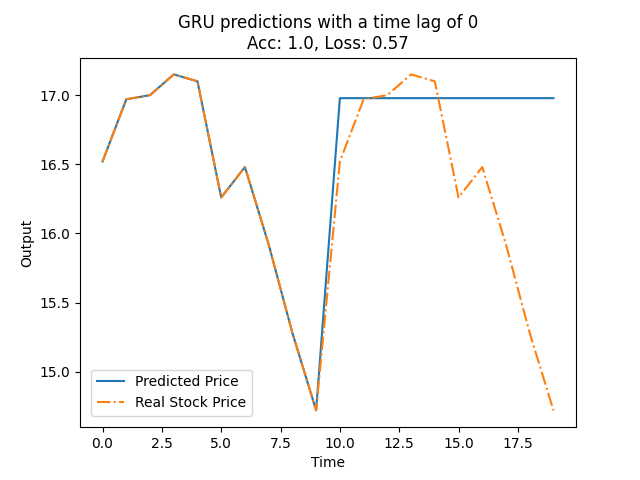
\includegraphics[width=\linewidth]{images/gruEval}
        \caption{The results from our GRU model}\label{Fig:gruEval}
    \end{minipage}\hfill
    \begin{minipage}{0.49\textwidth}
        \centering
        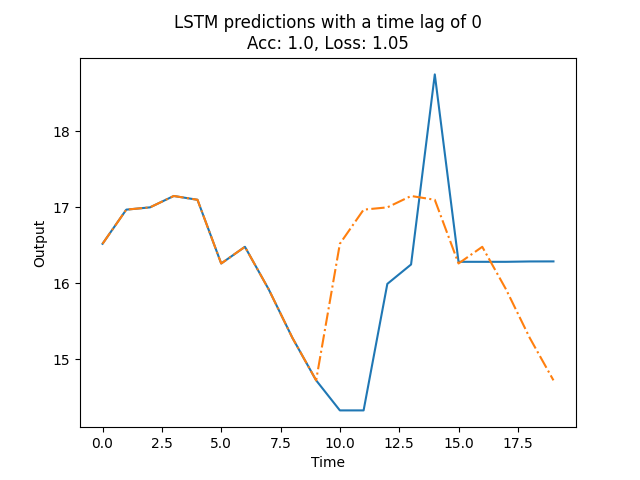
\includegraphics[width=\linewidth]{images/lstmEval}
        \caption{The results from our LSTM model}\label{Fig:lstmEval}
    \end{minipage}
\end{figure}

\begin{figure}[H]
    \begin{minipage}{0.49\textwidth}
        \centering
        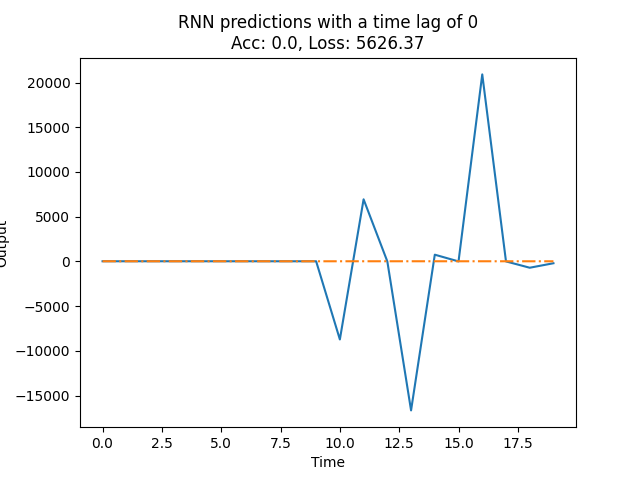
\includegraphics[width=\linewidth]{images/rnnEval}
        \caption{The results from our RNN model}\label{Fig:rnnEval}
    \end{minipage}\hfill
    \begin{minipage}{0.49\textwidth}
        \centering
        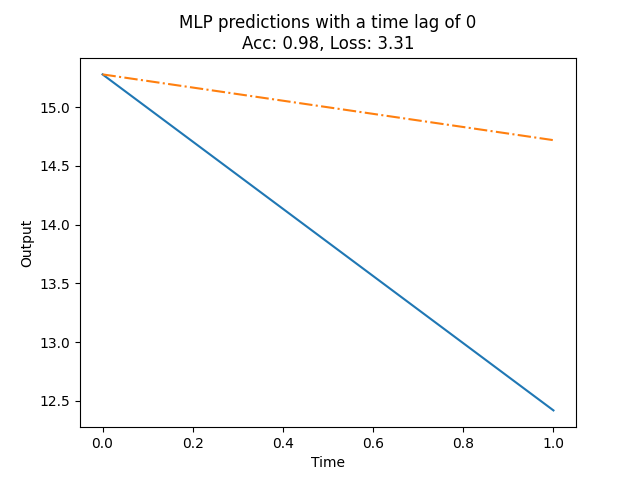
\includegraphics[width=\linewidth]{images/mlpEval}
        \caption{The results from our MLP model}\label{Fig:mlpEval}
    \end{minipage}
\end{figure}

Each of these results reflects the individual strengths and weaknesses of each model.  As is reflected in our
\textit{model\_complexity} calculations, the GRU model is the most performant, with a loss of only 0.57.  This is closely
followed by the LSTM model, which still offers a good prediction, but is slightly less consistent overall. In our
evaluation of our RNNs, we noticed a good example of the exploding gradients problem.  Without the limits provided by
the GRU and LSTM models, the predictions of the RNN become increasingly erratic.  Finally, our MLP model does not suffer
from an exploding gradient, but it does lack the recurrence of the other three models, only being able to output one day
at a time.

\subsection{End-To-End Testing}

The final component of our testing was the end-to-end series of tests we performed.  The goal of these tests was to give
us a holistic picture of how well our project functioned and how well that functioning met our stated goals.
For all of these tests, we started with front-end user interaction and ended with the response to those actions.

\paragraph{Price Queries}
The first and most straightforward set of operations that we tested were the three price query operations.
We performed this test by submitting query requests on the front end, then tracing the functions called by that operation
from the client to the oracle, then to the oracle getting the price, then finally back to the client.  We performed this
test for all three of our queries, testing different sets of inputs, both valid and invalid, to see if they were handled
properly.

\paragraph{Major Transactions}
The next set of tests we performed focused on our major transactions: \textit{Upload Dataset}, \textit{Train Model}, and
\textit{Query Model}.  These tests were similar to those for the price queries.  As we performed these tests, we noted
that, while the operations did complete successfully, the user feedback and results were ambiguous.  Additionally, we
realized that it might be confusing for the user to remember the exact names of the models and datasets in order to use
them.  To address these issues, we made several additions.  To address the issue of users having to input the exact names,
we added a dropdown feature instead of a test input.  We now store a list of the system's current datasets and models.
This is updated upon the reloading of the page or when a user submits a transaction.  This ensures the list is always
updated for better ease of use.  To address the feedback issue, we added a feedback section that periodically pinged the
client to see if any new response transactions came in from the oracle.  If these transactions did come in, we would
display the operation, the model or dataset name, and any extra data (like the result of a query) to the user.  This way,
the user would not have to check the transaction note on the Algorand block explorer manually.

By performing these tests, we were able to both evaluate the quality of the project as a whole and make important additions
to improve the user experience.  Our transaction tests helped us to identify the issues that had previously existed and
to verify that the current communication protocol was working properly.  Our model tests helped us to confirm our previous
assumptions about the nature of our various models and which scenarios they are most useful in.  Finally, our end-to-end
testing confirmed the overall functioning of the project and inspired us to make some valuable improvements to the user
experience.

\section{Conclusion}

\subsection{Summary}

Throughout our work, we have made PredictChain into a functional blockchain-based marketplace for predictive AI models.
Through PredictChain, users are now able to upload datasets for training predictive models, request that basic models be
trained on any previously uploaded datasets, or submit queries to those trained models. A central node with computing
resources available will operate these various models. A variety of
models are available, ranging from cheap, fast, and simple to more expensive, slower, and more powerful. This will allow
for a large variety of predictive abilities for both simple and complex patterns.  All the past predictions from these
models will be stored on the blockchain for public viewing.

\subsection{Future Work}

As mentioned above, we have several opportunities for improvement that could be accomplished with future work on this
project.  One major improvement that we could make to the project is giving users who upload datasets greater flexibility
in how their data is preprocessed.  This may come in the form of some feature engineering, similar to that found in Shen
and Shafiq(2020)~\cite{deepPrediction}.  Another potential improvement that could be introduced with future work is adding
a greater variety of models or more example datasets.  Currently, we only use neural networks to use for predictions.
In future work, we would like to add a more diverse set of models, such as decision trees or more statistical models based
on Bayesian inference.  Finally, we could make improvements to how our models are trained, for instance, allowing users
to prune off attributes from a dataset that they did not deem useful to the trained model.  Adding these improvements may
make PredictChain a more fleshed-out version without changing our project's core principles.

\ledgernotes

\section*{Acknowledgements} 

We would like to thank Professor Oshani Seneviratne for her guidance and support on this project.
We would also like to thank Rensselaer Polytechnic Institute.

\section*{Author Contributions}

MTP developed the bulk of the back end code, including the oracle, the client, the models, and the dataset management.
CJP worked, primarily, with the front end and user interface along with important contributions to client integration.

% \section*{Conflict of Interest}


%AUTHOR: comment out if using thebibliography
%\theendnotes

%AUTHOR: please read ledgerbib.bst usage notes by opening it in a text editor. We have modified it to include the use of the @misc item type for the proper formatting of online sources.

\pagebreak

\bibliographystyle{ledgerbib}
\bibliography{main}

%AUTHOR: comment out, this is used to make sure the Creative Commons License
%image fits on page

%\newpage 	
%define the following sections to have the Appendix Style

%\appendix
%\setcounter{section}{0}
%\section{Data and Descriptions}

%\vspace{12pt}
%\begin{table}[h]
%\begin{center} 
%\scalebox{0.6}{ 
%\begin{tabular}{p{5cm}p{18cm}}%{l|}%{|>m{5cm}|>m{15cm}|}
%\rowcolor{orange}
%\hline
% \textbf{Column A}  & \textbf{Column B} \\\hline
%	Data & Description of data in more detail.\\
%\hline
 %Also Data & More description of data.\\
%\hline 
 %A Third Item & Pretium fusce id velit ut tortor pretium viverra suspendisse potenti. Enim sed faucibus turpis in eu. In hac habitasse %platea dictumst quisque sagittis. Pharetra et ultrices neque ornare aenean euismod elementum.\\
%\hline
%\hline
%\end{tabular}}
%\caption{A table in an appendix} \label{AppendixTable}
%\end{center}
%\end{table} 
%\newpage
%here up^^


\thispagestyle{pagelast}

%\theendnotes

\end{document}
